\documentclass[10pt,a5paper,openany,fancyhdr]{memoir}
\usepackage[left=2cm,right=2cm,top=2cm,bottom=2cm]{geometry}
\usepackage[utf8x]{inputenc}
\usepackage[bahasa]{babel}
\usepackage{amsmath}
\usepackage{amsfonts}
\usepackage{amssymb}
\usepackage{palatino}
\usepackage{xspace}
\usepackage{verse}

%\author{Yohanes Suyanto}
\author{Gereja St Anna -- Duren Sawit \\  
Jakarta Timur}
\title{Ibadat Kematian\\ 
dan \\
Peringatan Arwah \\
{~}\\
\vspace{2cm}
~\\
(Edisi Percobaan) \\
~\\
sekretariat\_stanna@yahoo.com \\
~\\
~\\
}
\date{2009}
\setlength{\parindent}{0mm}
\makeatletter
\newcommand{\lagu}[1]{%
  {\parindent \z@ 
    \interlinepenalty\@M \slshape \mdseries \large \textit{#1}\par\nobreak \vskip 10\p@ }}
\newcommand{\keterangan}[1]{%
  {\parindent \z@ 
    \interlinepenalty\@M \slshape \mdseries \textit{#1}\par\nobreak \vskip 10\p@ }}
\makeatother

\newcommand{\BU}[1]{\begin{itemize}\itemsep0pt \item[U:] #1 \end{itemize}}
\newcommand{\BI}[1]{\begin{itemize}\itemsep0pt \item[I:] #1 \end{itemize}}
\newcommand{\BIU}[1]{\begin{itemize}\itemsep0pt \item[I+U:] #1 \end{itemize}}
\newcommand{\BPU}[1]{\begin{itemize}\itemsep0pt \item[P+U:] #1 \end{itemize}}
\newcommand{\BP}[1]{\begin{itemize}\itemsep0pt \item[P:] #1 \end{itemize}}

\newcommand{\inputlagu}[1]{\begin{textit} \input{#1} \end{textit}}

\newcommand{\nama}{Bapak VF Parlan\xspace}

\newlength\chaptitlelength
\newlength\chaptitlerlength

\makeatletter 
\newcommand\thickhrulefill[1]{%
  \leavevmode \leaders \hrule height #1 \hfill \kern \z@} 
\setlength\midchapskip{10pt} 
\makechapterstyle{mystyle}{
  \setlength\beforechapskip{0pt}
  \renewcommand\chapternamenum{} 
  \renewcommand\printchaptername{}
  \renewcommand\printchapternum{} 
  \renewcommand\chaptitlefont{\small\scshape\centering}
  \renewcommand*{\printchaptertitle}[1]{%
    \settowidth\chaptitlelength{\hspace*{1em}\chaptitlefont##1\hspace*{1em}}%
    \ifnum\chaptitlelength>\dimexpr0.7\textwidth\relax%
      \setlength\chaptitlelength{0.7\textwidth}%
    \fi%
    \setlength\chaptitlerlength{\textwidth}%
    \addtolength\chaptitlerlength{-\chaptitlelength}%
    \addtolength\chaptitlerlength{-2em}%
    \noindent\parbox[c]{.5\chaptitlerlength}{\normalsize\thickhrulefill{0.3ex}\par\vskip-1.5ex\thickhrulefill{0.2ex}}\hspace*{1em}%
    \parbox[c]{\chaptitlelength}{\chaptitlefont##1}\hspace*{1em}%
    \parbox[c]{.5\chaptitlerlength}{\normalsize\thickhrulefill{0.3ex}\par\vskip-1.5ex\thickhrulefill{0.2ex}}%
  }%
}
\makeatother
\chapterstyle{mystyle}
\chapterstyle{wilsondob}
\setcounter{secnumdepth}{2}

\begin{document}
\pagestyle{Ruled}
\begin{titlingpage}
\maketitle
\end{titlingpage}

Kematian merupakan peristiwa iman. Pada saat kematian, kita mengambil 
bagian dalam misteri Paskah Kristus. Bersama Yesus Kristus kita beralih 
dari dunia fana ke dalam kehidupan kekal. Kematian adalah pintu masuk ke 
dalam pemurnian diri manusia menuju pada keabadian. Kematian juga 
menghantar kita pada kepenuhan hidup di dalam dan bersama Kristus 
Tuhan kita. 

 



%Daftar Isi 
\renewcommand{\cftchapterfont}{\normalfont\rmfamily}   
\renewcommand{\cftsectionfont}{\normalfont\rmfamily}   
\newpage
\tableofcontents



\chapter{IBADAT PERINGATAN ARWAH HARI KE-40} 
\documentclass[a5paper,headsepline,titlepage,11pt,nnormalheadings,DIVcalc]{scrbook}
\usepackage[a5paper,backref]{hyperref}
\usepackage[papersize={148.5mm,215mm},twoside,bindingoffset=0.5cm,hmargin={2cm,2cm},
				vmargin={2cm,2cm},footskip=1.1cm,driver=dvipdfm]{geometry}
\usepackage{palatino}
\usepackage{graphicx}
\usepackage{wrapfig}
\usepackage[bahasa]{babel}
\usepackage{fancyhdr}
\usepackage{longtable}
\usepackage{hhline,multirow}
\usepackage{pst-node}

\renewcommand{\footrulewidth}{0.5pt}
\lhead[\fancyplain{}{\thepage}]%
      {\fancyplain{}{~}}
\rhead[\fancyplain{}{~}]%
      {\fancyplain{}{\thepage}}
\pagestyle{fancy}
\lfoot[\emph{Doa 40 hari \namaalm}]{}
\rfoot[]{\emph{Lingkungan St Petrus Maguwo}}
\cfoot{}

\newcommand{\BU}[1]{\begin{itemize} \item[U:] #1 \end{itemize}}
\newcommand{\BI}[1]{\begin{itemize} \item[I:] #1 \end{itemize}}
\newcommand{\BP}[1]{\begin{itemize} \item[P:] #1 \end{itemize}}
\newcommand{\BPP}[1]{\begin{itemize} \item[Bpk:] #1 \end{itemize}}
\newcommand{\BPW}[1]{\begin{itemize} \item[Ibu:] #1 \end{itemize}}
\newcommand{\namaalm}{Bapak Vincentius Muharto~}
\newcommand{\namaromo}{~}
\title{Ibadat/Doa untuk Arwah}
\author{}
\date{2011}
\hyphenation{a-kan}
\hyphenation{ba-gi-mu}
\hyphenation{ber-a-da}
\hyphenation{ber-du-a}
\hyphenation{be-ri-kan}
\hyphenation{ber-ka-ta}
\hyphenation{ber-nya-nyi}
\hyphenation{ber-sa-ma}

\hyphenation{dah-syat}
\hyphenation{DA-RAH-KU}
\hyphenation{da-tang}
\hyphenation{di-ka-ta-kan}
\hyphenation{di-pim-pin}
\hyphenation{di-se-rah-kan}
\hyphenation{di-tum-pah-kan}

\hyphenation{Eng-kau}
\hyphenation{ha-dap-an}
\hyphenation{han-tar-kan-lah}
\hyphenation{ha-rap-an}

\hyphenation{ja-lan}
\hyphenation{ja-ngan-lah}

\hyphenation{ka-nak}
\hyphenation{ka-re-na}
\hyphenation{kau-lim-pah-kan}
\hyphenation{Kau-cip-ta-kan}
\hyphenation{ke-bang-kit-an-Nya}
\hyphenation{ke-da-tang-an}
\hyphenation{ke-da-tang-an-Nya}
\hyphenation{ke-dua}
\hyphenation{ke-na-ik-kan-nya}
\hyphenation{ke-pa-daMu}
\hyphenation{ke-ra-him-an}
\hyphenation{ke-se-jah-te-ra-an-mu}
\hyphenation{ko-men-tar}

\hyphenation{la-ma-nya}
\hyphenation{lim-pah-kan}

\hyphenation{ma-nu-sia}
\hyphenation{me-nga-da-kan}
\hyphenation{me-ngan-dung-lah}
\hyphenation{me-ngu-kuh-kan}
\hyphenation{me-la-lui}
\hyphenation{me-lim-pah-kan}
\hyphenation{me-lu-hur-kan}
\hyphenation{me-me-cah-me-cah-kan}
\hyphenation{mem-per-sem-bah-kan}
\hyphenation{me-nan-da-ta-ngan-i}
\hyphenation{men-cin-tai}
\hyphenation{meng-a-lir-kan}
\hyphenation{me-nga-sihi}
\hyphenation{me-nge-lu-ar-kan}
\hyphenation{meng-u-cap-kan}
\hyphenation{meng-ung-kap-kan}
\hyphenation{me-num-buh-kan}
\hyphenation{me-nya-ta-kan}
\hyphenation{me-nye-la-mat-kan}
\hyphenation{me-nye-rah-kan}
\hyphenation{me-nye-rah-kanNya}
\hyphenation{me-ra-ya-kan}

\hyphenation{o-rang}
\hyphenation{o-rang-o-rang}

\hyphenation{pa-sang-kan-lah}
\hyphenation{pa-tut}
\hyphenation{pe-ne-ri-ma-an}
\hyphenation{pe-ngam-pun-an}
\hyphenation{Pe-ngan-ta-ra}
\hyphenation{peng-hi-bur-an}
\hyphenation{per-bu-at-an-nya}
\hyphenation{per-ka-ta-an}
\hyphenation{per-ka-win-an}
\hyphenation{per-ni-kah-an}
\hyphenation{per-se-ku-tu-an}
\hyphenation{per-sem-bah-an}
\hyphenation{rom-bong-an}

\hyphenation{se-la-ma}
\hyphenation{se-ka-li-an}
\hyphenation{se-pan-jang}
\hyphenation{se-ra-ya}
\hyphenation{Su-dar-yan-to}

\hyphenation{te-ta-pi}
\hyphenation{ta-ngan-Mu}
\hyphenation{Tu-han}
\hyphenation{tu-lang}
\hyphenation{tu-lang-tu-lang}

\hyphenation{u-mat-Mu}
\hyphenation{wa-kil}

\hyphenation{ba-gi-mu}
\hyphenation{di-se-rah-kan}
\hyphenation{me-la-lui}
\hyphenation{ka-nak}
\hyphenation{ka-re-na}
\hyphenation{ber-ka-ta}
\hyphenation{te-ta-pi}
\hyphenation{per-ka-win-an}
\hyphenation{pa-tut}
\hyphenation{me-lu-hur-kan}
\hyphenation{ber-nya-nyi}
\hyphenation{di-tum-pah-kan}
\hyphenation{pe-ngam-pun-an}
\hyphenation{ber-a-da}
\hyphenation{kau-lim-pah-kan}
\hyphenation{ke-bang-kit-an-Nya}
\hyphenation{per-ka-ta-an}
\hyphenation{pa-sang-kan-lah}
\hyphenation{DA-RAH-KU}
\hyphenation{ke-na-ik-kan-nya}
\hyphenation{per-sem-bah-an}
\hyphenation{per-se-ku-tu-an}


\renewcommand*\thesection{\arabic{section}.}
\setlength{\parindent}{0mm} 

\begin{document}
\thispagestyle{empty}
%\maketitle
%\newsavebox\IBox
%\sbox\IBox{\includegraphics[scale=0.4]{Saint-Peter-Apostle-e.eps}}

\psset{unit=1in}
\begin{pspicture}(4in,6.0in)
% set up the fonts we use
\DeclareFixedFont{\PT}{T1}{ppl}{b}{it}{0.4in}
\DeclareFixedFont{\PTsmall}{T1}{ppl}{b}{it}{0.3in}
\DeclareFixedFont{\PTsmallest}{T1}{ppl}{b}{it}{0.2in}
\DeclareFixedFont{\PTtext}{T1}{ppl}{b}{it}{11pt}
\DeclareFixedFont{\Logo}{T1}{pbk}{m}{n}{0.2in}
% place the front cover picture
%\rput[cb](2.3,2.5){\usebox\IBox}
% put the text on the front cover
\rput[cb](2.5,5.3){\PTsmall {Ibadat/Doa Arwah 40 hari untuk}}
\rput[cb](2.5,4.8){\PTsmall {\namaalm}}
\rput[cb](2.5,1.1){\PTsmall {8 November 2011}}
\rput[cb](2.5,0.6){\PTsmallest {Wilayah Yohanes de Britto}}
\rput[cb](2.5,0.3){\PTsmallest {Stasi Maguwo}}
\rput[cb](2.5,0.0){\PTsmallest {Paroki Marganingsih Kalasan }}

%\rput[cb](3,-1){\PTsmallest {\namagereja}} 

\end{pspicture}
%\tableofcontents 
\newpage
\thispagestyle{empty}
{~}
\newpage
\setlength{\parskip}{2mm}

\section*{RITUS PEMBUKA}
\subsection*{LAGU PEMBUKA}

\subsection*{SALAM PEMBUKAAN}
\BP{Atas nama Bapa Putera dan Roh Kudus} 
\BU{Amin}
\BP{Semoga damai sejahtera Tuhan kita Yesus Kristus, cinta kasih Allah Bapa dan persekutuan Roh Kudus, selalu beserta kita.}
\BU{Sekarang dan selama-lamanya}

\subsection*{PENGANTAR}
\BP{Bapak, Ibu, Saudara Saudari yang terkasih dalam Kristus, 40 hari yang lalu keluarga ini mengalami duka yang mendalam. Kalau ditanya mengapa berduka? Jawabanya adalah karena pada waktu itu \namaalm telah dipanggil Tuhan. Mungkin kita bisa ikut merasakan perasaan / suasana hati dari keluarga yang ditinggalkan pada waktu itu. Sebagai ungkapan cinta keluarga ini terhadap almarhumah \namaalm kita semua diundang untuk bersama-sama mendukung dengan doa-doa supaya arwah dari \namaalm segera dapat ikut bangkit mulia bersama Kristus di dalam kerajaan surga.}

\emph{Hening sejenak \dots}
  
\subsection*{PERNYATAAN TOBAT}
\BP{Saudara-saudari yang seiman dalam Kristus, marilah kita membuat diri pantas berada di depan hadirat Allah, dengan membersihkan diri kita dari dosa dan kesalahan yang lalu, dengan bertobat dan mohon ampun kepada Allah kita.}

\BP{Saya mengaku \dots}

\BP{Semoga Allah yang mahakuasa mengasihani kita, 
mengampuni dosa kita dan mengantar kita ke dalam hidup 
yang kekal.}

\BU{Amin}

\subsection*{Tuhan Kasihanilah Kami}

\subsection*{Doa Pembuka}
\BP{Marilah Berdoa 

Allah Bapa yang mahamurah, Engkau telah menyerahkan 
Yesus, Putra-Mu kepada kematian, semua ini harus terjadi 
untuk melepaskan kami dari segala kuasa kegelapan dan 
dosa. Ya Bapa, anugerahkanlah hidup kekal kepada 
\namaalm yang telah menghadap 
kehadiratMu 40 hari yang lalu. Ya Bapa, ampunilah 
segala dosa dan kesalahannya dan bukalah pintu 
kehidupan kekal baginya. Terimalah saudara kami 
tercinta ini kedalam keluarga kudusMu di tahta surgawi. }

\BU{Amin} 
 
\section*{IBADAT SABDA}
\BP{Saudara-saudari terkasih marilah kita mempersiapkan hati 
dan budi untuk mendengarkan sabda Tuhan.} 

\subsection*{BACAAN PERTAMA}

\BP{Pembacaan dari 1 Kor 15:12-18 

Saudara-saudara bilamana kami beritakan, bahwa Kristus dibangkitkan dari antara orang mati, bagaimana mungkin ada di antara kamu yang mengatakan, bahwa tidak ada kebangkitan orang mati?
Kalau tidak ada kebangkitan orang mati, maka Kristus juga tidak dibangkitkan.

Tetapi andaikata Kristus tidak dibangkitkan, maka sia-sialah pemberitaan kami dan sia-sialah juga kepercayaan kamu.
Lebih dari pada itu kami ternyata berdusta terhadap Allah, karena tentang Dia kami katakan, bahwa Ia telah membangkitkan Kristus?padahal Ia tidak membangkitkan-Nya, kalau andaikata benar, bahwa orang mati tidak dibangkitkan.

Sebab jika benar orang mati tidak dibangkitkan, maka Kristus juga tidak dibangkitkan.
Dan jika Kristus tidak dibangkitkan, maka sia-sialah kepercayaan kamu dan kamu masih hidup dalam dosamu.
Demikianlah binasa juga orang-orang yang mati dalam Kristus. 

Demikianlah sabda Tuhan }

\BU{Syukur kepada Allah} 

\subsection*{LAGU TANGGAPAN} 

\subsection*{Bacaan Injil} 

\BP{Tuhan beserta kita} 
\BU{Sekarang dan selama-lamanya} 
\BP{Inilah Injil Yesus Kristus menurut Yohanes (6:37-40) 

Semua yang diberikan Bapa kepada-Ku akan datang kepada-Ku, dan barangsiapa datang kepada-Ku, ia tidak akan Kubuang.
Sebab Aku telah turun dari sorga bukan untuk melakukan kehendak-Ku, tetapi untuk melakukan kehendak Dia yang telah mengutus Aku.

Dan Inilah kehendak Dia yang telah mengutus Aku, yaitu supaya dari semua yang telah diberikan-Nya kepada-Ku jangan ada yang hilang, tetapi supaya Kubangkitkan pada akhir zaman.
Sebab inilah kehendak Bapa-Ku, yaitu supaya setiap orang, yang melihat Anak dan yang percaya kepada-Nya beroleh hidup yang kekal, dan supaya Aku membangkitkannya pada akhir zaman.

Demikianlah Injil Tuhan} 

\BU{Terpujilah Kristus}

\subsection*{HOMILI}

``Semua yang telah diberikan-Nya kepada-Ku jangan ada yang hilang, tetapi supaya Kubangkitkan pada akhir zaman.''


Pada hari ini kita diajak untuk mengenangkan \namaalm yang telah dipanggil Tuhan 40 hari yang lalu. Dalam rangka mengenangkan orang yang telah dipanggil Tuhan mungkin kita lalu ingat cara hidup dan cara bertindak mereka, nasihat dan saran mereka, kenakalan, kelucuan mereka dst \ldots Kami percaya bahwa kita akan mengingat-ingat apa yang baik, mulia, luhur dan indah yang dihayati oleh \namaalm yang telah meninggalkan kita. Kiranya kita semua memiliki harapan, sebagaimana disabdakan oleh Yesus, yaitu semoga ``semua yang telah diberikan-Nya kepada-Ku jangan ada yang hilang, tetapi supaya Kubangkitkan pada akhir zaman''. Maka marilah pada hari ini kita mawas diri perihal iman dan harapan kita.

\begin{quote}
\textit{Semua yang diberikan Bapa kepada-Ku akan datang kepada-Ku, dan barangsiapa datang kepada-Ku, ia tidak akan Kubuang. Sebab Aku telah turun dari sorga bukan untuk melakukan kehendak-Ku, tetapi untuk melakukan kehendak Dia yang telah mengutus Aku. Dan Inilah kehendak Dia yang telah mengutus Aku, yaitu supaya dari semua yang telah diberikan-Nya kepada-Ku jangan ada yang hilang, tetapi supaya Kubangkitkan pada akhir zaman} (Yoh 6:37-39)
\end{quote}

Semua orang kiranya berkendak baik, namun karena situasi lingkungan hidup dimana kita dilahirkan dan dibesarkan berbeda satu sama lain, maka tidak mustahil kehendak baik kita berbeda satu sama lain atau bahkan saling berlawanan; terjadi pemahaman atau pengertian perihal ‘apa yang baik’ berbeda-beda. Dengan kata lain masing-masing diri kita memiliki keterbatan-keterbatasan atau kelemahan-kelemahan, dan hanya karena kasih dan kemurahan hati Allah kita akhirnya dapat melakukan apa yang lebih baik daripada apa yang kita bayangkan atau pikirkan. Demikianlah kita mengenal mereka yang hidup dekat dengan kita dan telah dipanggil Tuhan, dan mungkin kita tahu kelemahan dan kekuatan, kekurangan dan kelebihannya, serta kita ragu-ragu apakah yang bersangkutan hidup mulia selamanya bersama Allah di sorga kembali. Marilah kita imani kasih dan kemurahan hati Allah.

Dasar iman kita akan kasih dan kemurahan hati Allah adalah sabda Yesus di puncak kayu salib dalam menanggapi permohonan/doa salah seorang penjahat yang disalibkan bersama-Nya ``Aku berkata kepadamu, sesungguhnya hari ini juga engkau akan ada bersama-sama dengan Aku di dalam Firdaus.'' (Luk 23:43). Karena keterbatasan dirinya ada kemungkinan orang berkehendak baik namun dalam perilakunya tidak baik, maka orang yang demikian ini pada detik-detik terakhir hidupnya akan berdoa seperti salah seorang penjahat yang disalibkan bersama-Nya ``Yesus, ingatlah akan aku, apabila Engkau datang sebagai Raja.'' (Luk 23:42). Kejahatan yang dilakukannya karena keterbatasan dirinya atau lingkungan hidupnya. Maka marilah kita imani bahwa saudara-saudari kita yang telah meninggal dunia telah hidup mulia kembali di sorga bersama Allah selamanya karena kasih dan kemurahan hati-Nya.

Kita semua yang masih hidup kiranya juga berharap bahwa setelah meninggal dunia nanti akan hidup mulia selamanya di sorga. Maka marilah kita wujudkan harapan kita dengan gairah, gembira dan dinamis melaksanakan aneka nasihat dan saran dari mereka yang telah meninggal dunia atau meneladan cara hidup dan cara bertindaknya yang baik. Dengan kata lain kita tidak terpisahkan dari mereka yang telah meninggal dunia jika kita hidup bersama dan bersatu dengan Tuhan. Harapan kita wujudkan dengan melaksanakan semua kehendak Tuhan seoptimal dan sebaik mungkin, dan kiranya usaha tersebut akan berhasil jika kita bekerjasama. Maka sebagaimana kita hari ini berdosa bersama-sama, marilah kita wujudkan kebersamaan tersebut dalam cara hidup dan cara bertindak kita setiap hari.

\begin{quote}
\textit{Jadi, bilamana kami beritakan, bahwa Kristus dibangkitkan dari antara orang mati, bagaimana mungkin ada di antara kamu yang mengatakan, bahwa tidak ada kebangkitan orang mati? Kalau tidak ada kebangkitan orang mati, maka Kristus juga tidak dibangkitkan} (1Kor 15:12-13)
\end{quote}

Sebagai orang beriman kita percaya akan kebangkitan orang mati di akhir zaman, apalagi orang yang beriman kepada Yesus Kristus. Dengan kata lain kita percaya kepada apa yang belum atau tidak kelihatan, itulah ciri khas orang beriman. Dengan kata lain beriman berarti tidak hidup dan bertindak secara materialistis, hanya mengandalkan diri pada yang kelihatan dan tidak percaya kepada Yang Ilahi. Memang percaya kepada yang tak kelihatan pada umumnya juga membuat percaya kepada yang kelihatan semakin handal dan tangguh. Sebagai orang beriman percaya kepada apa yang kelihatan, entah itu manusia, binatang atau tanaman atau harta benda dan percaya kepada Yang Ilahi bagaikan mata uang bermuka dua, dapat dibedakan namun tak dapat dipisahkan.

Tanda bahwa kita percaya kepada Yang Ilahi antara lain ketika kita menghadapi tugas berat, tantangan, hambatan serta masalah kita akan tetap tegar, gembira, ceria, bersemangat dan dinamis, karena Allah senantiasa menyertai dan mendampingi hidup dan perjalanan kita. Sendirian di tengah malam kelam di jalanan atau di rumah pun juga tak takut dan tak gentar, karena ditemani oleh Allah. Aneka tantangan, hambatan, masalah dan tugas berat justru membangkitkan dan menggairahkan cara hidup dan cara bertindak kita, maka orang sungguh beriman suka akan tantangan, hambatan, masalah dan tugas-tugas berat. Ia akan berusaha mencari celah-celah guna mengatasi atau menerobos masalah, tantangan, hambatan dan tugas berat tersebut. Masalah, tantangan, hambatan dan tugas berat menjadi wahana perkembangan dan pertumbuhan.

Orang beriman yang percaya kepada kebangkitan bagaikan kecambah yang sedang tumbuh dan ditutupi dengan dedauan atau jerami, dimana ia justru semakin tumbuh alias tambah tinggi atau besar serta terus berusaha menatap sang matahari, pemberi kehidupan. Maka orang beriman akan mencari celah-celah di tengah kekacauan dan keributan untuk menemukan Allah, dengan kata lain mencari dan menemukan apa yang baik, kekuatan dan kesempatan guna mengatasi kekacauan atau keributan yang sedang berlangsung. Orang Jawa mengenal 'tapa ngrame' yang maksudnya bertapa dengan cara mengembara dan menolong sesama yang dijumpainya dan sedang mengalami kesulitan. Orang beriman dapat ‘tapa ing rame’, menemukan Tuhan dalam keramaian dan keributan. Ia mengusahakan kesucian hidup dengan sungguh mendunia, membumi, berpartisipasi dalam seluk-beluk duniawi di bumi ini. Ia sungguh penyelamat yang menyelamatkan apa yang tidak selamat.

\section*{DOA}

\subsection*{DOA UMAT}

\BP{Allah Bapa kami yang maha kasih dan penyayang, kami menghadap hadiratmu untuk menyampaikan ungkapan hati dan permohonan kami. Kami percaya Engkau akan selalu berkenan menyertai kami, mendengarkan kami dan memberikan yang terbaik bagi kami. Kami memuji dan memuliakan nama-Mu melalui doa-doa ini:}

\BP{Ya Tuhan Yesus Kristus penyelamat dunia kami mempercayakan kepadamu arwah \namaalm, berkenanlah engkau menerimanya dalam sukacita kerajaan-Mu

Kami mohon}

\BU{Kabulkanlah doa kami ya Tuhan}

\BP{Ya Allah, kami mohon kemurahaanmu bagi \namaalm , janganlah kau ingat-ingat lagi dosa-dosanya, tetapi limpahkanlah kerahiman-Mu kepadanya. Semoga Ia disambut dan dipersatukan bersama para malaikat dan orang kudus di surga.

Kami mohon}

\BU{Kabulkanlah doa kami ya Tuhan}

\BP{Bagi keluarga yang ditinggalkan, ya Bapa tolonglah mereka semua supaya saling mendukung , saling memberi kekuatan dan penghiburan. Semoga kenangan akan masa hidup \namaalm akan tersimpan dalam hati mereka, dan meneguhkan kepercayaan mereka akan bimbingan-Mu 

Kami mohon}

\BU{Kabulkanlah Doa kami ya Tuhan} 

\BP{Ya Bapa Keluarga ini telah menyerahkan seluruh hidupnya kedalam penyelenggaraan-Mu, maka sudilah mendampingi mereka supaya sanggup menghadapi liku-liku hidup ini , lebih-lebih saat ini dikala keluarga ini ditinggalkan oleh sosok Bapak yang mereka cintai.

Kami mohon}

\BU{Kabulkanlah doa kami ya Tuhan}

\BP{Bagi kita semua yang berhimpun disini beserta keluarganya, ya Bapa jadikanlah kami alat-Mu dalam menciptakan kerukunan dan penghiburan dan pembawa damai. Jauhkanlah kami semua dari kemalangan.

Kami mohon}

\BU{Kabulkanlah doa kami ya Tuhan}

\BP{Demikianlah ya Bapa, doa-doa yang kami panjatkan. Engkau mengetahui keinginan keinginan dan kesulitan kami. Kami percaya akan penyelenggaraan-Mu dan bersama Roh Kudus, kami senantiasa belajar utuk memahami apa yang sebenarnya Engkau kehendaki atas diri kami . Kami menyampaikan doa-doa kami ini dengan perantaraan Putera-Mu terkasih, Tuhan kami Yesus Kristus, yang hidup dan berkuasa kini dan sepanjang masa. Amin}


\subsection*{DOA BAPA KAMI}
Marilah kita satukan doa-doa permohonan kita dengan doa yang diajarkan Yesus sendiri 
Bapa kami yang ada di surga \dots .( didoakan bersama sama )

Ya Bapa terimah arwah \namaalm dalam kemuliaan kerajaan-Mu.

\section*{RITUS PENUTUP}

\subsection*{DOA PENUTUP}
\BP{Marilah berdoa :
 
Allah Bapa kami yang mahapengasih dan penyanyang, 
semoga kebangkitan putraMu juga menjadi kebangkitan 
saudara kami \namaalm  Bapa semoga Engkau senantiasa 
membangkitkan semangat kami untuk terus menerus hidup 
seturut nasihat InjilMu. Bapa, semoga doa-doa yang kami 
panjatkan kehadiratMu mampu mengantar saudara-saudari 
kami yang sudah meninggal untuk memasuki kerajaanMu 
yang abadi di surga. }
\BU{Amin} 

\subsection*{BERKAT}
\BP{Tuhan beserta kita}
\BU{Sekarang dan selama-lamanya}
\BP{Semoga kita semua, keluarga kita dan karya kita selalu di bimbing dan diberkati oleh Bapa dan Putera dan Roh Kudus.}

\BU{Amin}

\BP{Saudara sekalian ibadat kita sudah selesai marilah kita mundur dalam damai Tuhan}
\BU{Syukur kepada Allah.}

\subsection*{LAGU PENUTUP}

\end{document}

\chapter*{LAGU-LAGU PUJIAN}
\addcontentsline{toc}{chapter}{Lagu-lagu Pujian} 

\renewcommand{\thesection}{\arabic{section}.}
\renewcommand{\thesubsection}{\arabic{subsection}.}
\newlength{\saveleftmargini} % define a temp variable for the original margin
\setlength{\saveleftmargini}{\leftmargini} % write the original margin in this variable
\setsecnumdepth{subsection}

\subsection{TETAP CINTA YESUS} 
\begin{verse}
Kumau cinta Yesus selamanya \\
Kumau cinta Yesus selamanya \\
Meskipun badai silih berganti\\ 
Dalam hidupku\\ 
Kutetap cinta Yesus selamanya\\
\end{verse}
\begin{altverse}
Ya Bapa, Bapa ini aku anakMu \\
Layakkanlah seluruh hidupku \\
Ya Bapa, Bapa ini aku anakMu \\
Pakailah sesuai dengan rencanaMu
\end{altverse}

\subsection{KASIH DARI SURGA}
\begin{altverse}
Kasih dari surga memenuhi tempat ini \\
Kasih dari bapa surgawi \\
Kasih dari Yesus mengalir di hatiku \\
Membuat damai di hidupku 
\end{altverse}
\begin{verse}
Mengalir kasih dari tempat tinggi \\
Mengalir kasih dari tahta Allah Bapa \\
Mengalir, mengalir, mengalir dan mengalir \\
Mengalir memenuhi hidupku \\
\end{verse}

\subsection{KINI SAATNYA} 
\begin{altverse}
Kini saatnya berdiri di altarNya\\ 
S’bab Allah Maha Kudus hadir di sini\\ 
Marilah memuji angkat tangan menyembah\\ 
S’bab Allah Maha Kudus hadir di sini
\end{altverse}
\begin{verse}
Kita masuk tahta suciNya \\
Bersama para malaikat menyembah\\ 
Mari puji Yesusku \\
Kita masuk hadiratNya Maha Kudus 
\end{verse}

\subsection{SEJAUH TIMUR DARI BARAT} 
\begin{altverse}
Sejauh timur dari barat Engkau membuang dosaku\\ 
Tiada kau ingat lagi pelanggaranku\\ 
Jauh ke dalam tubir laut, Kau melemparkan dosaku\\ 
Tiada Kau perhitungkan kesalahanku 
\end{altverse}
\begin{verse}
Betapa besar kasih pengampunanMu, Tuhan\\ 
Tak Kau pandang hina hati yang hancur\\ 
Kuberterima kasih kepadaMu ya Tuhan \\
Pengampunan yang Kau bri pulihkanku 
\end{verse}

\subsection{BERI PENGAMPUNAN} 
\begin{altverse}
Dengan rendah hati aku mengaku \\
Atas dosaku s’lama ini \\
Ya Tuhan, Maha Pengasih \\
B’ri pengampunan untukku 
\end{altverse}
\begin{verse}
Kristus Putra bapa, Krsitus Juru S’lamat \\
Sungguh kusesali dosaku \\
Aku bersalah padaMu \\
B’ri pengampunan untukku 
\end{verse}

\subsection{KUSIAPKAN HATIKU TUHAN} 
\begin{altverse}
Kusiapkan hatiku tuhan ‘tuk dengar FirmanMu saat ini \\
Kusujud menyembahMu Tuhan Dalam hadiratMu saat ini 
\end{altverse}
\begin{verse}
Curahkan urapanMu Tuhan Bagi jemaatMu saat ini \\
Kusiapkan hatiku tuhan’tuk dengar FirmanMu 
\end{verse}
\begin{altverse}
\textit{Reff:} \\
FirmanMu Tuhan tiada berubah \\
Dahulu sekarang selama-lamanya, tiada berubah \\
FirmanMu Tuhan Penolong hidupku \\
Kusiapkan hatiku Tuhan ‘tuk dengar FirmanMu 
\end{altverse}

\subsection{FIRMANMU PELITA BAGI KAKIKU} 
\begin{altverse}
Firmanmu p’lita bagi kakiku terang bagi jalanku\\ 
FirmanMu p’lita bagi kakiku terang bagi jalanku 
\end{altverse}

\begin{verse}
Waktu kubimbang dan hilang jalanku \\
Tetaplah Kau di sisiku \\
Dan tak’kan ku takut sal Kau di dekatku\\ 
Besertaku selamanya 
\end{verse}


\subsection{BETAPA HATIKU} 
\begin{altverse}
Betapa hatiku berterima kasih Yesus,\\ 
Kau mengasihiku, Kau memilikiku
\end{altverse} 

\begin{verse}
Hanya ini Tuhan persembahanku, \\
Segenap hidupku jiwa dan ragaku \\
Sbab tak kumiliki harta kekayaan, \\
Yang cukup berarti ‘tuk kupersembahkan
\end{verse} 

\begin{altverse}
Hanya ini Tuhan permohonanku,\\ 
Terimalah Tuhan persembahanku \\
Pakailah hidupku sebagai alatMu,\\ 
Seumur hidupku
\end{altverse} 

\subsection{BAPA SURGAWI} 
\begin{altverse}
Bapa surgawi, ajarku mengenal \\
Betapa dalamnya kasihMu \\
Bapa surgawi buatku mengerti \\
Betapa kasihMu padaku
\end{altverse} 

\begin{verse}
Semua yang terjadi di dalam hidupku \\
Ajarku menyadari Kau selalu sertaku \\
Bri hatiku selalu, bersyukur padaMu \\
Karna rencanaMu indah bagiku
\end{verse} 

\subsection{BAYU SENJA} 
\begin{altverse}
Hidup bagai biduk di laut lepas \\
Aku pelaut tunggal siap melaju
\end{altverse}
 
\textit{Reff:} 
\begin{verse}
O bayu senja, hembusan sang Ilahi \\
Bawa bidukku ke tepian cerah \\
Pantai umat tebusan
\end{verse} 

\begin{altverse}
Arus gelombang tantang biduk tak daya \\
Hati merayu Tuhan nada nan cemas 
\end{altverse}

\textit{Reff}
 
\begin{verse}
Malam kabut nan pekat bintang pun lenyap\\ 
Setia kunanti Dikau wujud tak tampak \\
\textit{Reff}
\end{verse}
 

\subsection{ AVE MARIA}
\begin{altverse}
Engkau yang dipilih Allah Bapa di surga\\
Untuk melahirkan PutraNya yang kudus\\
Engkaulah Bunda Kristus\\
Bunda sang Penebus s’gala dosa manusia
\end{altverse}

\begin{verse}
Bunda Maria p’rawan yang tiada bernoda\\
Hatimu bersinar putih tiada bercela\\
Engkau Bunda Almasih yang diangkat\\
Ke surga penuh kemuliaan
\end{verse}

\begin{altverse}
Ave maria, ave Maria\\
Terpujilah Bunda, terpuji namaMu\\
S’panjang s’gala masa\\
Ave maria, ave Maria Syukur kepadaNya\\
Tuhan yang Pengasih S’lama-lamanya
\end{altverse}

\subsection{ TUHAN ADALAH GEMBALAKU}
\begin{altverse}
Tuhan adalah gembalaku, Tak’kan kekurangan aku\\
Ia membaringkan aku, Di padang yang berumput hijau
\end{altverse}

\begin{verse}
\textit{Reff:}\\
Ia membimbingku ke air yang tenang\\
Ia menyegarkan jiwaku\\
Ia menuntunku ke jalan yang benar\\
Oleh karna namaNya\\
Sekalipun aku berjalan, dalam lembah kekelaman
\end{verse}

\begin{altverse}
Aku tidak takut bahaya, Sebab Engkau besertaku\\
GadaMu dan tongkatMu, Itulah yang menghibur aku
\end{altverse}

\subsection{ KAU YANG TERINDAH}
\begin{altverse}
Kau yang terindah di dalam hidup ini\\
Tiada Allah Tuhan yang seperti Engkau\\
Besar perkasa penuh kemuliaan
\end{altverse}

\begin{verse}
Kau yang termanis di dalam hidup ini\\
Kucinta Kau lebih dari segalanya\\
Besar kasih setiaMu kepadaku
\end{verse}

\begin{altverse}
\textit{Reff:}\\
Kusembah Kau ya Allahku, Kutinggikan namaMu selalu\\
Tiada lutut tak bertelut, Menyembah Yesus Tuhan Rajaku
\end{altverse}

\begin{verse}
Kusembah Kau ya Allahku, Kutinggikan namaMu selalu\\
Selalu lidah kan mengaku, Engkaulah Yesus Tuhan Rajaku
\end{verse}

\subsection{ BAPA SURGAWI}
\begin{altverse}
Bapa surgawi ajarku mengenal\\
Betapa dalamnya kasihMu\\
Bapa surgawi buatku mengerti
\end{altverse}

\begin{verse}
Betapa kasihMu padaku\\
Semua yang terjadi, di dalam hidupku\\
Ajarku menyadari Kau selalu sertaku\\
Bri hatiku selalu, bersyukur padaMu\\
Karna rencanaMu indah bagiku
\end{verse}

\subsection{ ALLAH PEDULI}
\begin{altverse}
Banyak perkara yang tak dapat kumengerti\\
Mengapakah harus terjadi\\
Didalam kehidupan ini
\end{altverse}

\begin{verse}
Satu perkara yang kusimpan dalam hati\\
Tiada sesuatu kan terjadi tanpa Allah peduli
\end{verse}

\begin{altverse}
Allah mengerti, Allah peduli\\
Segala persoalan yang kita hadapi\\
Tak akan pernah dibiarkannya\\
Kubergumul sendiri\\
S’bab Allah peduli
\end{altverse}

\subsection{ ONE DAY AT THE TIME}
\begin{altverse}
I’m only human, I’m just a man\\
Help me believe in what I could be\\
And all that I am\\
Show me the stairway I have to climb\\
Lord for my sake; Teach me to take\\
One day at a time
\end{altverse}

\begin{verse}
\textit{Chorus:}\\
One day at a time sweet Jesus\\
That’s all I’m asking from you\\
Just give me a strength to do everything\\
What I have to do\\
Yesterday’s gone sweet Jesus\\
Tomorrow may never be mine
\end{verse}

\begin{verse}
Help me today show me the way\\
One daya at a time
\end{verse}

\begin{altverse}
Do you remember\\
When You walk among men\\
Well Jesus know\\
If you are looking below\\
It’s worst now and then\\
Cheating and stealing\\
Violence and crimed\\
So for may sake Lord teach me to take\\
One day at a time\\
\textit{back to chorus}
\end{altverse}

\subsection{ IN MOMENT LIKE THIS}
\begin{altverse}
In moment like this, I sing out a song\\
I sing out a love song to Jesus\\
In moment like this, I lift up my hands\\
I lift up my hands to the Lord
\end{altverse}

\subsection{ GIVE THANKS}
\begin{altverse}
Give thanks with a greatful heart\\
Give thanks to the Holy One\\
Give thanks because He’s given\\
Jesus Christ, His son:
\end{altverse}

\begin{verse}
And now let the weak say I’m strong\\
Let the poor say I’m rich\\
Because of what the Lord has done for us:\\
Give thanks

\end{verse}

\subsection{ TUBUHKU YESUS}
\begin{altverse}
TubuhMu Yesus sucikan daku\\
TubuhMu Yesus bebaskanku\\
TubuhMu Yesus ubahkan daku\\
Ku dijadikan baru
\end{altverse}

\subsection{ DARAHMU YESUS}
\begin{altverse}
DarahMu Yesus sucikan daku\\
DarahMu Yesus bebaskanku\\
DarahMu Yesus ubahkan adaku\\
Ku dijadikan baru
\end{altverse}

\subsection{ EL SHADAI}
\begin{altverse}
Tak usah ku takut, Allah menjagaku\\
Tak usah ku bimbang, Yesus p’liharaku\\
Tak usah ku susah, Roh Kudus hiburku\\
Tak usah ku cemas, Dia memberkatiku
\end{altverse}

\begin{verse}
El Shadai, El Shadai, Allah Maha kuasa\\
Dia besar, Dia besar, el Shadai mulia\\
El Shadai, El Shadai, Allah Maha kuasa\\
BerkatNya melimpah, El Shadai
\end{verse}

\subsection{ TIAP LANGKAHKU}
\begin{altverse}
Tiap langkahku diatur oleh Tuhan\\
Dan tangan kasihNya memimpinku\\
Di tengah badai dunia menakutkan\\
Hatiku tetap tenang teduh
\end{altverse}

\begin{verse}
\textit{Reff:}\\
Tiap langkahku ku tahu Tuhan yang pimpin\\
Ke tempat tinggi ku dihantarNya\\
Hingga sekali nanti aku tiba
\end{verse}

\begin{altverse}
Di rumah bapa, surga yang baka\\
Di waktu imanku mulai goyah\\
Dan bila jalanku hampir sesat
\end{altverse}

\begin{verse}
Kupandang Tuhanku Penebus dosa\\
Ku teguh sebab Dia dekat\\
\textit{Reff}
\end{verse}


\begin{altverse}
Di dalam tuhan saja harapanku\\
Sebab di tanganNya sejahtera\\
DibukaNya Yerusalem yang baru\\
Kota Allah yang suci mulia\\
\textit{Reff}
\end{altverse}



\subsection{ DI DOA IBUKU}
\begin{altverse}
Di waktuku masih kecil gembira dan senang\\
Tiada duka kukenal, tak kunjung mengerang\\
Di sore hari nan sepi ibuku bertelut\\
Sujud berdoa kudengar, namaku disebut
\end{altverse}

\begin{verse}
Seringlah ini kukenang di masa yan benar\\
Di kala hidup mendesak dan nyaris kusesat\\
Melintas gambar ibuku sewaktu bertelut\\
Kembali sayup kudengar namaku disebut
\end{verse}

\begin{altverse}
\textit{Reff:}\\
Di doa ibuku namaku disebut\\
Di doa ibu kudengar ada namaku disebut
\end{altverse}

\begin{verse}
Sekarang dia telah pergi ke rumah yang senang\\
Namun kasihnya padaku selalu kukenang\\
Kelak di sana kami pun bersama bertelut\\
Memuji Tuhan yang dengar namaku disebut\\
\textit{Reff}
\end{verse}

\subsection{ TUHAN BERIKANLAH}
\begin{altverse}
Tuhan berikanlah istirahat\\
Abadi dan tenang bagi yang wafat\\
Beri pengampunan segala dosanya\\
Karna Maha murah hatiMu Allah
\end{altverse}

\begin{verse}
Kami berimankan sabda Putra\\
Aku kebangkitan dan kehidupan\\
Barang siapalah percaya ‘kan daku\\
Ia akan hidup untuk selamanya
\end{verse}

\begin{altverse}
Kami menantikan saat itu\\
Maut akan lenyap diganti hidup\\
Smoga kami kelak memandang wajahMu\\
Di sinari terang dalam rumahMu
\end{altverse}

\subsection{ INDAH RENCANAMU TUHAN}
\begin{altverse}
Indah rencanaMU Tuhan di dalam hidupku\\
Walau ku tak tahu dan ku tak mengerti semua jalanMu\\
Dulu ku tak tahu Tuhan berat kurasakan\\
Hati menderita namun tak kuasa menghadapi semua
\end{altverse}

\begin{verse}
\textit{Reff:}\\
Tapi kumengerti s’karang Kau tolong padaku
\end{verse}

\subsection{ BAPA SUNGGUH BAIK}
\begin{altverse}
Bapa, Engkau sungguh baik\\
KasihMu melimpah di hidupku\\
Bapa, ku bert’rima kasih\\
BerkatMu hari ini, yang Kau sediakan bagiku
\end{altverse}

\begin{verse}
Kunaikkan syukurku buat hari yang Kau b’ri\\
Tak habis-habisnya kasih dan rahmatMu\\
Slalu baru dan tak pernah terlambat pertolonganMu\\
Besar setiaMu di s’panjang hidupku
\end{verse}

\subsection{ JALAN TUHAN}
\begin{altverse}
Ada waktu di hidupku\\
Pencobaan berat menekan\\
Aku berseru mengapa ya Tuhan\\
Nyatakan kehendakMu
\end{altverse}

\begin{verse}
Jalan Tuhan bukan jalanku\\
Jangan bimbang ataupun ragu\\
Nantikan tuhan jadikan semua\\
Indah pada waktunya
\end{verse}

\begin{altverse}
\textit{Reff:}\\
Pada Tuhan masa depanku\\
Pada Tuhan kus’rahkan hidupku\\
Nantikan Tuhan berkarya\\
Indah pada waktunya
\end{altverse}

\begin{verse}
Hari esok tiada kutahu\\
Namun tetap langkahku maju\\
Ku yakin Tuhan jadikan semua\\
Indah pada waktunya
\end{verse}

\subsection{ TANGAN TUHAN}
\begin{altverse}
Apa yang kau alami kini\\
Mungkin tak dapat engkau mengerti\\
Satu hal tanamkan di hati\\
Indah semua yang Tuhan beri
\end{altverse}

\begin{verse}
Tuhanku tak akan memberi\\
Ular beracun pada yang minta roti\\
Cobaan yang engkau alami\\
Tak melebihi kekuatanmu\\
\textit{Reff:}\\
Tangan Tuhan sedang merenda\\
Suatu karya yang agung mulia\\
Saatnya ‘kan tiba nanti\\
Kau lihat pelangi kasihNya
\end{verse}

\subsection{ HANYA KEPADAMU}
\begin{altverse}
Hanya kepadaMu kami dapat berpasrah\\
Tuhan Yesus Kristus\\
Di dalam tanganMu hidup dan mati kami\\
Engkaulah Penebus
\end{altverse}

\begin{verse}
CintaMu ya tuhan mengalahkan maut\\
Hanya Dikau pangkal kehidupan\\
Yang selalu kami dambakan
\end{verse}

\begin{altverse}
Ya Yesus sambutlah saudara kami ini\\
Dalam rumah Bapa\\
Karna Engkau wafat supaya kami hidup\\
Untuk selamanya
\end{altverse}

\begin{verse}
Hidup atau mati kami milik Tuhan\\
Maka Tuhan bimbinglah umatMu,\\ 
Di jalan menuju padaMu
\end{verse}

\subsection{ DOAKAN KAMI BUNDA}
\begin{altverse}
Cantik hatimu tiada bernoda\\
Bunda penolong umat manusia\\
Trimalah nyanyian puji bagimu\\
Kar’na kekagumanku pada iman dalam bening hatimu
\end{altverse}

\begin{verse}
Kau perawan suci nan lembut hati\\
Terberkati dalam rahmat Ilahi\\
Dengarkan selalu doaku O Bunda yang setia\\
Kaulah perantara doa kami pada Yesus PutraMu
\end{verse}

\begin{altverse}
\textit{Reff:}\\
Maria, Maria terpujilah engkau untuk selamanya\\
Doakan kami Bunda saat ini dan saat ajal nanti
\end{altverse}

\subsection{ BUNDA PEMBANTU ABADI}
\begin{altverse}
Pada wajahmu yang suci\\
Matamu nampak bening sejuk lembut\\
Kau pandang para abdimu berdoa\\
Oh Bunda pembantu abadi\\
Engkau pagku anakmu Yesus Putra Allah\\
Sumber suka dan duka hatimu\\
Hanya engkau sendirilah yang tahu\\
Pahit dan manisnya hidupku
\end{altverse}

\begin{verse}
Bukanlah kepadamu oh bunda\\
Pandangan penuh cintaNya tertuju\\
Salib dan tombak bengis dilihatNya\\
Oh Bunda pembantu abadi\\
Tangan Bunda dipegang didekapNya erat\\
Gambaran gelisah manusia\\
Bagaikan terbayang sengsara maut\\
Siksaan salah manusia
\end{verse}

\begin{altverse}
Matamu ya Bunda suci\\
Memberitakan pesanNyaterindah\\
Wahau kamu orang-orang berdosa\\
Lihatlah juru selamatmu\\
Terdengar pesan indah namun kami lemah\\
Terbawa gelombang masa kini\\
Kami pinta doamu pada Bapa\\
Oh Bunda Pembantu abadi
\end{altverse}

\begin{verse}
Pandanglah dunia ini oh bunda\\
Dunia yang penuh dengan kebencian\\
Doakan perdamaian yang sejati\\
Sadarkan hati manusia\\
Arahkan pikian tingkah laku kami\\
Biarkan tampak cinta sesame\\
Bantulah di saat ajalku tiba\\
Oh Bunda Pembantu abadi


\end{verse}


\end{document}

